\chapter{Analisis}
\label{chap:analisis}

Bab ini membahas hasil analisis berdasarkan dasar teori yang sudah dijelaskan sebelumnya. Pada bab ini dijelaskan hasil analisis \textit{dataset} yang digunakan dalam pengujian, representasi dokumen dalam perangkat lunak, dan pemodelan ruang vektor pada dokumen. Selain itu pada bab ini juga dibahas mengenai representasi kromosom, fungsi \textit{fitness}, dan beberapa operasi genetik yang digunakan dalam membuat pengelompokan dokumen berbasis algoritma genetika.

\section{Analisis \textit{Dataset}}
\label{sec:dataset}
Pada bagian ini dibahas mengenai \textit{dataset} yang digunakan dalam proses pengujian. \textit{Dataset} yang digunakan berisi artikel berita \textit{BBC News} dan disediakan untuk menjadi tolok ukur dalam penelitian pembelajaran mesin. Karakteristik dari \textit{dataset} ini antara lain:

\begin{itemize}
	\item Terdiri dari 2225 dokumen yang berasal dari \textit{website BBC News} dari tahun 2004-2005.
	\item Dokumen ditulis dalam Bahasa Inggris.
	\item Terbagi menjadi lima topik yaitu \textit{business, entertainment, politics, sport}, dan \textit{tech}.
	\item Pada topik \textit{business} terdapat 510 dokumen, \textit{entertainment} terdapat 386 dokumen, \textit{politics} terdapat 417 dokumen, \textit{sport} terdapat 511 dokumen, dan \textit{tech} terdapat 401 dokumen.
	\item Dokumen merupakan \textit{plain text} yang ditulis dalam file dengan ekstensi \textit{TXT}.
	\item Rata-rata dalam satu dokumen terdapat 384 kata.
\end{itemize}

Dokumen-dokumen ini kemudian akan diproses terlebih dahulu untuk membersihkan tanda baca dalam dokumen (hanya mengambil informasi berupa karakter alfanumerik). Selain itu, seluruh kapitalisasi dalam dokumen akan diabaikan (setiap huruf kapital akan diubah ke dalam huruf kecil). Contoh dokumen untuk setiap topik (\textit{business, entertainment, politics, sport}, dan \textit{tech}) dilampirkan pada Lampiran \ref{lamp:C}

\section{Representasi Dokumen}
\label{sec:document-rep}
Dokumen tidak bisa langsung digunakan begitu saja dalam proses pengelompokan. Tidak seperti manusia yang dapat melakukan proses secara manual, komputer tidak dapat menemukan nilai informasi dari data mentah berupa dokumen. Dokumen yang ada perlu direpresentasikan menjadi bentuk yang bisa diambil informasinya baru kemudian dapat diolah dalam proses lebih lanjut. Model ruang vektor (Subbab \ref{sec:vsm}) digunakan dalam penelitian ini untuk merepresentasikan dokumen sehingga informasinya dapat diproses dengan lebih mudah.

\section{Model Ruang Vektor}
\label{sec:analysis:vsm}
Pada subbab \ref{sec:vsm} telah dijelaskan bahwa dokumen akan dibentuk ke dalam sebuah vektor yang memiliki banyak dimensi berdasarkan banyaknya \term berbeda dalam dokumen. Seperti yang telah dibahas pada subbab \ref{sec:termWeight}, ada dua cara untuk menentukan bobot dari suatu \term dalam dokumen yaitu bobot frekuensi dan bobot tf-idf. Sebagai contoh akan digunakan tiga dokumen berikut:

\begin{enumerate}
	\item Penjualan properti di Indonesia meningkat di Bulan Februari.
	\item Penjualan asuransi kendaraan di Indonesia meningkat.
	\item Bulan Februari merupakan bulan puncak penjualan kendaraan.
\end{enumerate}

Berdasarkan tiga dokumen tersebut maka ditentukan bobot dari masing-masing \textit{term} dalam tiap dokumen untuk setiap jenis pembobotan.

\subsection{Bobot Frekuensi}
Pada subbab \ref{sub:freq} telah dijelaskan bahwa bobot frekuensi dari suatu \term dapat ditentukan dengan cara menghitung banyaknya kemunculan \term tersebut dalam dokumen. Hasil perhitungan bobot frekuensi berdasarkan contoh pada Subbab \ref{sec:analysis:vsm} ditunjukkan dalam Tabel \ref{tbl:freq}.

\begin{table}[h]
	\centering
	\caption{Hasil perhitungan bobot frekuensi}
	\begin{tabular}{|c|c|c|c|} \hline
		\multirow{2}{*}{\Term} & \multicolumn{3}{c|}{Bobot} \\ \cline{2-4}
		& Dokumen 1 & Dokumen 2 & Dokumen 3 \\ \hline 
        penjualan & 1 & 1 & 1 \\ \hline
        properti & 1 & 0 & 0 \\ \hline
        di & 2 & 1 & 0 \\ \hline
        indonesia & 1 & 1 & 0 \\ \hline
        meningkat & 1 & 1 & 0 \\ \hline
        bulan & 1 & 0 & 2 \\ \hline
        februari & 1 & 0 & 1 \\ \hline
        asuransi & 0 & 1 & 0 \\ \hline
        kendaraan & 0 & 1 & 1 \\ \hline
        merupakan & 0 & 0 & 1 \\ \hline
        puncak & 0 & 0 & 1 \\ \hline
	\end{tabular}
	\label{tbl:freq}
\end{table}

Semakin besar nilai bobot, maka \term dianggap semakin mewakili isi dokumen. Sebagai contoh pada Tabel \ref{tbl:freq}, \term "di" muncul dua kali pada dokumen 1 sehingga berbobot 2, muncul satu kali pada dokumen 2 sehingga berbobot 1, dan tidak muncul sama sekali pada dokumen 3 sehingga memiliki bobot 0. \Term "di" dianggap mewakili dokumen 1 karena muncul dua kali pada dokumen tersebut.

\subsection{Bobot TF-IDF}
\label{sub:analysis:tf-idf}
Berbeda dengan bobot frekuensi yang hanya menghitung frekuensi kemunculan \term pada dokumen, perhitungan bobot TF-IDF ini memerlukan perhitungan seperti yang telah dijelaskan dalam Persamaan \ref{eq:tf-idf} pada Subbab \ref{sub:tf-idf}. Sama dengan perhitungan bobot frekuensi, contoh yang berasal dari Subbab \ref{sec:analysis:vsm} digunakan sebagai ilustrasi perhitungan TF-IDF. Sesuai dengan apa yang telah dijelaskan pada Subbab \ref{sub:tf-idf}, perhitungan dari TF-IDF akan dibagi menjadi dua tahap yaitu perhitungan TF dan perhitungan IDF. 

\Term "properti" akan digunakan dalam contoh perhitungan TF. Berdasarkan Persamaan \ref{eq:tf} pada Subbab \ref{sub:tf-idf}, maka perhitungan TF dari \term "properti" ditunjukkan pada Persamaan \ref{eq:tf-idf:tf}.

\begin{equation}
	\label{eq:tf-idf:tf}
	\begin{gathered}
 	%\textrm{tf}_{t,d}=\frac{\textrm{f}_{t,d}}{\sum_{t' \in d}\textrm{f}_{t',d}} \\
	\textrm{tf}_{"properti",1}=\frac{1}{8}=0.125
	\end{gathered}
\end{equation}

Penjelasan dari Persamaan \ref{eq:tf-idf:tf} adalah sebagai berikut. $\textrm{f}_{"properti",1}$ bernilai 1 karena \term "properti" hanya muncul 1 kali pada dokumen 1. Dokumen 1 terdiri dari 8 \term sehingga $\textrm{tf}_{"properti",1}$ bernilai $0.125$. Berdasarkan Persamaan \ref{eq:tf-idf:tf}, maka hasil perhitungan TF dari ketiga dokumen tersebut ditunjukkan pada Tabel \ref{tbl:tf-idf:tf}.

\begin{table}[H]
	\centering
	\caption{Hasil perhitungan TF}
	\begin{tabular}{|c|c|c|c|} \hline
		\multirow{2}{*}{\Term} & \multicolumn{3}{c|}{Bobot} \\ \cline{2-4}
		& Dokumen 1 & Dokumen 2 & Dokumen 3 \\ \hline 
        penjualan & 0.1250 & 0.1667 & 0.1429  \\ \hline
        properti & 0.1250 & 0 & 0  \\ \hline
        di & 0.2500 & 0.1667 & 0  \\ \hline
        indonesia & 0.1250 & 0.1667 & 0  \\ \hline
        meningkat & 0.1250 & 0.1667 & 0  \\ \hline
        bulan & 0.1250 & 0 & 0.2857  \\ \hline
        februari & 0.1250 & 0 & 0.1429  \\ \hline
        asuransi & 0 & 0.1667 & 0  \\ \hline
        kendaraan & 0 & 0.1667 & 0.1429  \\ \hline
        merupakan & 0 & 0 & 0.1429  \\ \hline
        puncak & 0 &	0 &	0.1429  \\ \hline
	\end{tabular}
	\label{tbl:tf-idf:tf}
\end{table}

Untuk perhitungan IDF digunakan Persamaan \ref{eq:idf} pada Subbab \ref{sub:tf-idf}. Perhitungan IDF untuk \term "properti" ditunjukkan oleh Persamaan \ref{eq:tf-idf:idf}.

\begin{equation}
	\label{eq:tf-idf:idf}
	\begin{gathered}
	%\textrm{idf}_t = \textrm{log} \frac{N}{\textrm{df}_t} \\
	\textrm{idf}_{"properti"}=\textrm{log} \frac{3}{1}=0.4771
	\end{gathered}
\end{equation}

Penjelasan dari Persamaan \ref{eq:tf-idf:idf} adalah sebagai berikut. $N$ bernilai 3 karena banyaknya dokumen dalam seluruh koleksi dokumen adalah 3. $\textrm{df}_t$ bernilai 1 karena hanya ada 1 dokumen yang memuat \term "properti" yaitu dokumen 1. Hasil dari perhitungan IDF untuk setiap \term ditunjukkan oleh Tabel \ref{tbl:tf-idf:idf}.

\begin{table}[H]
	\centering
	\caption{Hasil perhitungan IDF}
	\begin{tabular}{|c|c|} \hline
		\Term & IDF \\ \hline 
        penjualan & 0 \\ \hline
        properti & 0.4771 \\ \hline
        di & 0.1761 \\ \hline
        indonesia & 0.1761 \\ \hline
        meningkat & 0.1761 \\ \hline
        bulan & 0.1761 \\ \hline
        februari & 0.1761 \\ \hline
        asuransi & 0.4771 \\ \hline
        kendaraan & 0.1761 \\ \hline
        merupakan & 0.4771 \\ \hline
        puncak & 0.4771 \\ \hline
	\end{tabular}
	\label{tbl:tf-idf:idf}
\end{table}

\Term penjualan pada Tabel \ref{tbl:tf-idf:idf} bernilai 0. \Term "penjualan" muncul di ketiga dokumen sehingga pada saat perhitungan IDF menghasilkan nilai nol ($log \frac{N}{N_i}=log \frac{3}{3} = 0$). Dapat disimpulkan bahwa \term "penjualan" tidak mewakili dokumen manapun karena muncul di semua dokumen.

Hasil dari perhitungan TF dan IDF digabung dengan cara dikalikan. Perhitungan TF-IDF untuk \term "properti" pada dokumen 1 ditunjukkan dalam Persamaan \ref{eq:tf-idf:complete}.

\begin{equation}
	\label{eq:tf-idf:complete}
	\begin{gathered}
	\textrm{tf-idf}_{t,d} = \textrm{tf}_{t,d} \times \textrm{idf}_t \\
	\textrm{tf-idf}_{"properti",1} = 0.125 \times 0.4771 = 0.0075
	\end{gathered}
\end{equation}

Nilai yang berasal dari Persamaan \ref{eq:tf-idf:tf} dan Persamaan \ref{eq:tf-idf:idf} dikalikan sehingga didapatkan hasil sesuai dengan Persamaan \ref{eq:tf-idf:complete}. Hasil perhitungan TF-IDF untuk seluruh \term dalam ketiga dokumen ditunjukkan dalam Tabel \ref{tbl:tf-idf}.

\begin{table}[H]
	\centering
	\caption{Hasil perhitungan bobot TF-IDF}
	\begin{tabular}{|c|c|c|c|} \hline
		\multirow{2}{*}{\Term} & \multicolumn{3}{c|}{Bobot} \\ \cline{2-4}
		& Dokumen 1 & Dokumen 2 & Dokumen 3 \\ \hline 
        penjualan & 0 & 0 & 0 \\ \hline
        properti & 0.0075 & 0 & 0 \\ \hline
        di & 0.0055 & 0.0049 & 0 \\ \hline
        indonesia & 0.0028 & 0.0049 & 0 \\ \hline
        meningkat & 0.0028 & 0.0049 & 0 \\ \hline
        bulan & 0.0028 & 0 & 0.0072 \\ \hline
        februari & 0.0028 & 0 & 0.0036 \\ \hline
        asuransi & 0 & 0.0133 & 0 \\ \hline
        kendaraan & 0 & 0.0049 & 0.0036 \\ \hline
        merupakan & 0 & 0 & 0.0097 \\ \hline
        puncak & 0 & 0 & 0.0097 \\ \hline
	\end{tabular}
	\label{tbl:tf-idf}
\end{table}

\section{Representasi Kromosom}
\label{sec:chromosome-rep}
Individu dalam pengelompokan merupakan salah satu cara pengelompokan. Dalam penelitian ini, individu direpresentasikan oleh sebuah kromosom. Kromosom tersusun dari gen-gen yang merupakan \textit{centroid} dari $K$ buah \textit{cluster} yang akan dibentuk. \textit{Centroid} disimpan dalam bentuk vektor yang terdiri dari $N$ buah bilangan riil. $N$ merupakan dimensi dari vektor tersebut yang merupakan banyaknya \term berbeda yang terdapat pada seluruh koleksi dokumen. Oleh karena itu, setiap kromosom akan memiliki $N\times K$ buah gen. Meskipun \textit{centroid} menyimpan informasi mengenai isi dari dokumen, namun \textit{centroid} belum tentu merupakan sebuah dokumen. \textit{Centroid} dapat berupa suatu vektor pada bidang $N$ dimensi yang merupakan titik tengah dari suatu \textit{cluster}. Secara umum representasi \textit{centroid} ke dalam kromosom ditunjukkan pada Gambar \ref{fig:chromosome-rep}.

\begin{figure}[H]
	\centering
	\begin{tabular}{c c c c}
		$C_1$ & $C_2$ & & $C_k$ \\
		$w_{1,1}, w_{1,2}, ..., w_{1,n}$, & $w_{2,1}, w_{2,2}, ..., w_{2,n}$ & ... & $w_{k,1}, w_{k,2}, ..., w_{k,n}$
	\end{tabular}
	\caption{Formula representasi kromosom}
	\label{fig:chromosome-rep}
\end{figure}

Berdasarkan Gambar \ref{fig:chromosome-rep}, $N$ gen pertama merepresentasikan $N$ dimensi dari \textit{centroid} pertama $C_1$ ($w_{1,1}, w_{1,2}, ..., w_{1,n}$), $N$ gen selanjutnya merepresentasikan $N$ dimensi dari \textit{centroid} kedua $C_2$ ($w_{2,1}, w_{2,2}, ..., w_{2,n}$), dan seterusnya sampai \textit{centroid} $C_k$ ($w_{k,1}, w_{k,2}, ..., w_{k,n}$). Sebagai contoh apabila diketahui ada tiga buah \textit{centroid} dalam bidang dua dimensi $\mathbf{C1}$ (3.05, 1.43), $\mathbf{C2}$ (15.85, 14.23), dan $\mathbf{C3}$ (5.12, 9.45). Hasil representasi ketiga \textit{centroid} pada kromosom ditunjukkan oleh Gambar \ref{fig:chromosome}.

\begin{figure}[H]
	\centering
	\begin{tabular}{|c|c|c|c|c|c|}
		\multicolumn{2}{c}{\textbf{$\mathbf{C1}$}} & \multicolumn{2}{c}{\textbf{$\mathbf{C2}$}} & \multicolumn{2}{c}{$\mathbf{C3}$}\\ \hline
		3.05 & 1.43 & 15.85 & 14.23 & 5.12 & 9.45\\ \hline
	\end{tabular}
	\caption{Contoh representasi \textit{centroid} ke dalam kromosom}
	\label{fig:chromosome}
\end{figure}

\section{Fungsi \textit{Fitness}}
\label{sec:func-fitness-analysis}
Seperti yang telah dijelaskan pada Subbab \ref{sec:chromosome-rep}, kromosom akan tersusun atas \textit{centroid} yang berbentuk vektor. Oleh karena itu, perhitungan \textit{fitness} akan mengalami beberapa penyesuaian. Perhitungan \textit{fitness} dalam penelitian ini terdiri dari tiga tahap. Pada tahap pertama, terjadi pembentukan \textit{cluster} berdasarkan titik pusat yang terkandung dalam kromosom. Hal ini dilakukan dengan menetapkan setiap dokumen $x_i,i=1,2, ... ,n$ ke dalam sebuah \textit{cluster} $C_j$ dengan \textit{centroid} $z_j$ sehingga memenuhi Persamaan \ref{eq:minimum-dist}.

\begin{equation}
\label{eq:minimum-dist}
\Vert x_i-z_j \Vert < \Vert x_i-z_p \Vert , p=1,2, ... ,K \mbox{, dan } p \neq j.
\end{equation}

Persamaan \ref{eq:minimum-dist} menjelaskan bahwa akan dicari suatu \textit{cluster} $C_j$ yang paling dekat dengan dokumen $x_i$. Hal ini dilakukan dengan cara membandingkan jarak antara dokumen $x_i$ dengan seluruh \textit{centroid} dari $K$ buah \textit{cluster}. 

Setelah proses pengelompokan selesai, maka dilanjutkan dengan tahap kedua yaitu mengganti \textit{centroid} terkandung dalam kromosom dengan \textit{centroid} baru. \textit{Centroid} baru ini ditentukan dengan cara menghitung rata-rata vektor dari tiap \textit{cluster}. Untuk \textit{cluster} $C_i$, \textit{centroid} baru $z_i^*$ dapat dihitung menggunakan Persamaan \ref{eq:centroid}.

\begin{equation}
\label{eq:centroid}
z_i^*=\frac{1}{n_i} \sum_{x_j\in C_i} x_j,   i=1,2, ... ,K.
\end{equation}

dengan $z_i^*$ merupakan \textit{centroid} dari \textit{cluster} $i$, $n_i$ merupakan jumlah anggota \textit{cluster} $i$, dan $x_j$ merupakan dokumen $j$ yang merupakan anggota dari \textit{cluster} $i$. $z_i^*$ ini akan menggantikan $z_i$ sebelumnya di kromosom. 

Tahap terakhir dari perhitungan \textit{fitness} adalah menghitung nilai \textit{fitness} itu sendiri. Pada penelitian ini, nilai \textit{fitness}  dihitung menggunakan \textit{cosine similarity} seperti yang sudah dijelaskan pada Subbab \ref{sec:vsm}. Sesuai dengan Persamaan \ref{eq:intracluster} pada Subbab \ref{sec:metric}, perhitungan \textit{fitness} sebagai metrik yang menggambarkan seberapa baiknya suatu calon solusi ditunjukkan dalam Persamaan \ref{eq:cosSim-fitness} dengan beberapa penyesuaian.
\begin{equation}
\label{eq:cosSim-fitness}
	\begin{gathered}
	\textrm{f}=\sum_{i=1}^K \textrm{f}_i , \\
	\textrm{f}_i=\sum_{x_j\in C_i}\dfrac{x_j\cdot z_i}{\parallel x_j \parallel \times \parallel z_i \parallel}
	\end{gathered}
\end{equation}

Penjelasan dari Persamaan \ref{eq:cosSim-fitness} adalah sebagai berikut. Nilai \textit{fitness} $\textrm{f}$ didapatkan dengan menjumlahkan nilai \textit{fitness} $\textrm{f}_i$ setiap \textit{centroid} $i=1, 2, ..., K$. Nilai \textit{fitness} $\textrm{f}_i$ tiap \textit{centroid} didapatkan dengan menjumlahkan jarak setiap dokumen ke \textit{centroid} masing-masing (Subbab \ref{sec:metric}). Perhitungan jarak antara dokumen dengan \textit{centroid} dihitung dengan menggunakan \textit{cosine similarity} sehingga persamaan untuk menghitung \textit{cosine similarity} (Persamaan \ref{eq:cosine} pada Subbab \ref{sec:vsm}) dimasukkan ke dalam Persamaan \ref{eq:cosSim-fitness}. Semakin besar nilai \textit{fitness} $\textrm{f}$, maka kromosom tersebut semakin mendekati solusi yang optimal.

\section{Operasi Genetik Dalam Pengelompokan Dokumen}
\label{sec:gen-op}
Seperti yang telah di bahas pada Subbab \ref{sec:GA}, ada beberapa operator genetik yang digunakan dalam algoritma genetika. Beberapa operasi genetik yang digunakan dalam penelitian ini di antaranya adalah inisialisasi populasi, seleksi, persilangan, dan mutasi. Sama seperti kromosom, operator genetik ini juga perlu dimodifikasi sedemikian rupa sehingga dapat digunakan untuk proses pengelompokan dokumen. Berikut merupakan pembahasan lebih detil mengenai setiap operator genetik yang digunakan.

\subsection{Inisialisasi Populasi}
\label{sub:analysis:pop-init}
Proses pengelompokan dengan menggunakan algoritma genetika dimulai dengan inisialisasi populasi awal. Seperti yang sudah dijelaskan pada Subbab \ref{sec:chromosome-rep}, kromosom dari masing-masing individu terdiri dari $K$ buah \textit{centroid} dalam bentuk vektor. Populasi awal dibangkitkan dengan cara memilih $K$ dokumen secara acak yang kemudian dijadikan \textit{centroid} mula-mula. Kemudian proses tersebut dilakukan sebanyak $P$ kali dengan $P$ adalah banyaknya individu dalam populasi.

\subsection{Seleksi}
\label{sub:analysis:selection}
Proses seleksi dilakukan setiap iterasi (setiap generasi) untuk memilih calon induk dari generasi selanjutnya. Pada penelitian ini digunakan teknik seleksi \textit{roulette-wheel selection} seperti yang telah dijelaskan pada Subbab \ref{sub:selection}. \textit{Roulette-wheel selection} digunakan secara langsung pada penelitian ini dan tidak dimodifikasi. Individu dengan nilai \textit{fitness} lebih tinggi memiliki probabilitas lebih tinggi untuk terpilih menjadi induk dari generasi selanjutnya dan masuk ke dalam proses persilangan. Namun karena masih ada peluang individu dengan nilai \textit{fitness} tertinggi tidak terpilih, maka dalam penelitian ini juga digunakan teknik elitisme \cite{ahn2003elitism}. Dengan digunakannya elitisme, maka individu dengan nilai \textit{fitness} terbaik disalin dan langsung menjadi anggota dari generasi berikutnya. Hal ini dilakukan untuk menjamin individu terbaik tidak hilang akibat tidak terpilih oleh \textit{roulette-wheel selection}.

\subsection{Persilangan}
\label{sub:analysis:crossover}
Dua kromosom yang terpilih dalam proeses seleksi disilangkan untuk menghasilkan keturunan yang akan dimasukkan ke dalam generasi selanjutnya. Dalam penelitian ini akan digunakan teknik persilangan dengan satu titik potong (\textit{single-point crossover}). Teknik \textit{single-point crossover} yang digunakan dalam penelitian ini sedikit berbeda karena perlu disesuaikan dengan kebutuhan pengelompokan dokumen. Titik potong tidak ditentukan pada tingkat gen, namun ditentukan pada tingkat \textit{centroid}. Apabila diketahui terdapat kromosom seperti pada Gambar \ref{fig:ilust-crossover:chromosome}, maka titik potong yang dipilih bukan berupa gen ($w_{k,n}$) melainkan \textit{centroid} ($C_k$).

\begin{figure}[H]
	\centering
	\begin{tabular}{c c c c c}
		$C_1$ & $C_2$ & $C_3$ & $C_4$ & $C_5$ \\
		$w_{1,1}, w_{1,2}, ..., w_{1,n}$, & $w_{2,1}, w_{2,2}, ..., w_{2,n}$, & $w_{3,1}, w_{3,2}, ..., w_{3,n}$, & $w_{4,1}, w_{4,2}, ..., w_{4,n}$, & $w_{5,1}, w_{5,2}, ..., w_{5,n}$
	\end{tabular}
	\caption{Ilustrasi kromosom untuk persilangan}
	\label{fig:ilust-crossover:chromosome}
\end{figure}

Sebagai contoh, diketahui dua buah kromosom yang mengalami persilangan adalah kromosom $A$ dengan kromosom $B$ seperti pada Gambar \ref{fig:illust-crossover}. Setelah itu ditentukan suatu titik potong (\textit{crossover point}) secara acak dan ditandai dengan garis tegak berwarna merah pada Gambar \ref{fig:illust-crossover}. Proses selanjutnya adalah pembentukan individu keturunan. Proses ini dilakukan dengan cara menggabungkan seluruh gen induk $A$ yang berada di sebelah kiri garis merah dengan seluruh gen induk $B$ yang berada di sebelah kanan garis merah. Keturunan yang dihasilkan dari proses ini hanya satu individu seperti yang dapat dilihat pada Gambar \ref{fig:illust-crossover}. 

\begin{figure}[H]
	\centering
	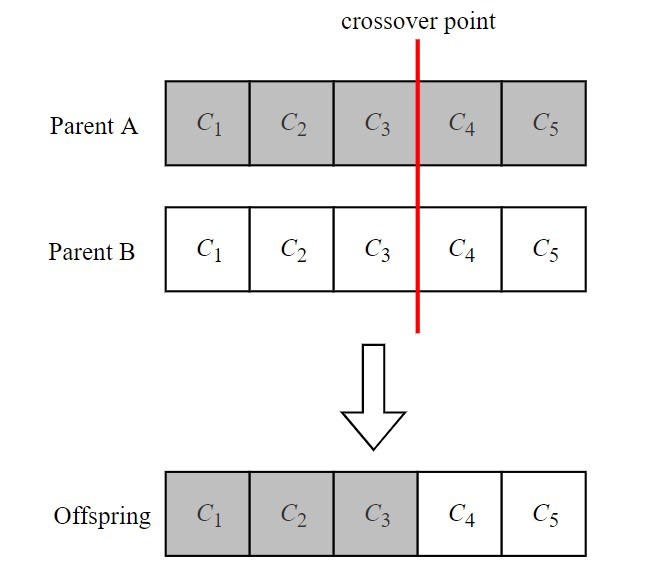
\includegraphics[width=0.5 \linewidth]{crossover}
	\caption{Ilustrasi persilangan}
	\label{fig:illust-crossover}
\end{figure}

\subsection{Mutasi}
\label{sub:analysis:mutation}
Setiap individu keturunan yang berasal dari proses persilangan memiliki peluang untuk mengalami mutasi. Seperti yang telah dijelaskan pada Subbab \ref{sub:mutation}, mutasi dapat terjadi berdasarkan peluang mutasi $\mu_m$. Apabila mutasi terjadi, maka akan ditentukan gen mana yang mengalami mutasi dengan mengambilnya secara acak. Nilai gen yang baru dapat ditentukan menggunakan Persamaan \ref{eq:mutation:analysis}.

\begin{equation}
	\label{eq:mutation:analysis}
	v'=v\pm 2*\delta*v
\end{equation}

dengan $v'$ nilai yang baru dari gen setelah mutasi, $v$ merupakan nilai gen sebelumnya, dan $\delta$ merupakan suatu bilangan acak antara 0 sampai 1 yang dibangkitkan menggunakan pesebaran \textit{uniform}. Sebagai contoh dengan menggunakan Gambar \ref{fig:mutated:before}, akan ditentukan satu dari enam gen yang akan mengalami mutasi. Misalkan dalam contoh ini gen kedua yang mengalami mutasi (Gambar \ref{fig:mutated:choose}). Setelah dilakukan perhitungan nilai menggunakan Persamaan \ref{eq:mutation:analysis}, kromosom hasil mutasi ditunjukkan dalam Gambar \ref{fig:mutated:after}.

\begin{figure}[H]
	\centering
	\begin{subfigure}[t]{\textwidth}
		\centering
		\begin{tabular}{|c|c|c|c|c|c|}
			\multicolumn{2}{c}{\textbf{$\mathbf{C1}$}} & \multicolumn{2}{c}{\textbf{$\mathbf{C2}$}} & \multicolumn{2}{c}{$\mathbf{C3}$}\\ \hline
		3.05 & 1.43 & 15.85 & 14.23 & 5.12 & 9.45\\ \hline
		\end{tabular}
		\caption{Kromosom sebelum mutasi}
		\label{fig:mutated:before}
	\end{subfigure}
	
	\vspace{5mm}
	\begin{subfigure}[t]{\textwidth}
		\centering
		\begin{tabular}{|c|c|c|c|c|c|}
			\multicolumn{2}{c}{\textbf{$\mathbf{C1}$}} & \multicolumn{2}{c}{\textbf{$\mathbf{C2}$}} & \multicolumn{2}{c}{$\mathbf{C3}$}\\ \hline
		3.05 & \textbf{1.43} & 15.85 & 14.23 & 5.12 & 9.45\\ \hline
		\end{tabular}
		\caption{Pemilihan gen yang akan dimutasi}
		\label{fig:mutated:choose}
	\end{subfigure}
	
	\vspace{5mm}
	\begin{subfigure}[t]{\textwidth}
		\centering
		\begin{tabular}{|c|c|c|c|c|c|}
			\multicolumn{2}{c}{\textbf{$\mathbf{C1}$}} & \multicolumn{2}{c}{\textbf{$\mathbf{C2}$}} & \multicolumn{2}{c}{$\mathbf{C3}$}\\ \hline
		3.05 & {\color{red} \textbf{2.59}} & 15.85 & 14.23 & 5.12 & 9.45\\ \hline
		\end{tabular}
		\caption{Kromosom hasil mutasi}
		\label{fig:mutated:after}
	\end{subfigure}
		\caption{Ilustrasi mutasi kromosom}
		\label{fig:mutated}
\end{figure}

%\section{Diagram Kelas}
%Berdasarkan hasil analisis dari masalah yang dihadapi, dibentuklah diagram kelas pada gambar \ref{fig:diagramkelas} sebagai gambaran dari perangkat lunak yang akan dibuat.
%
%\begin{figure}[h]
%	\begin{center}
%		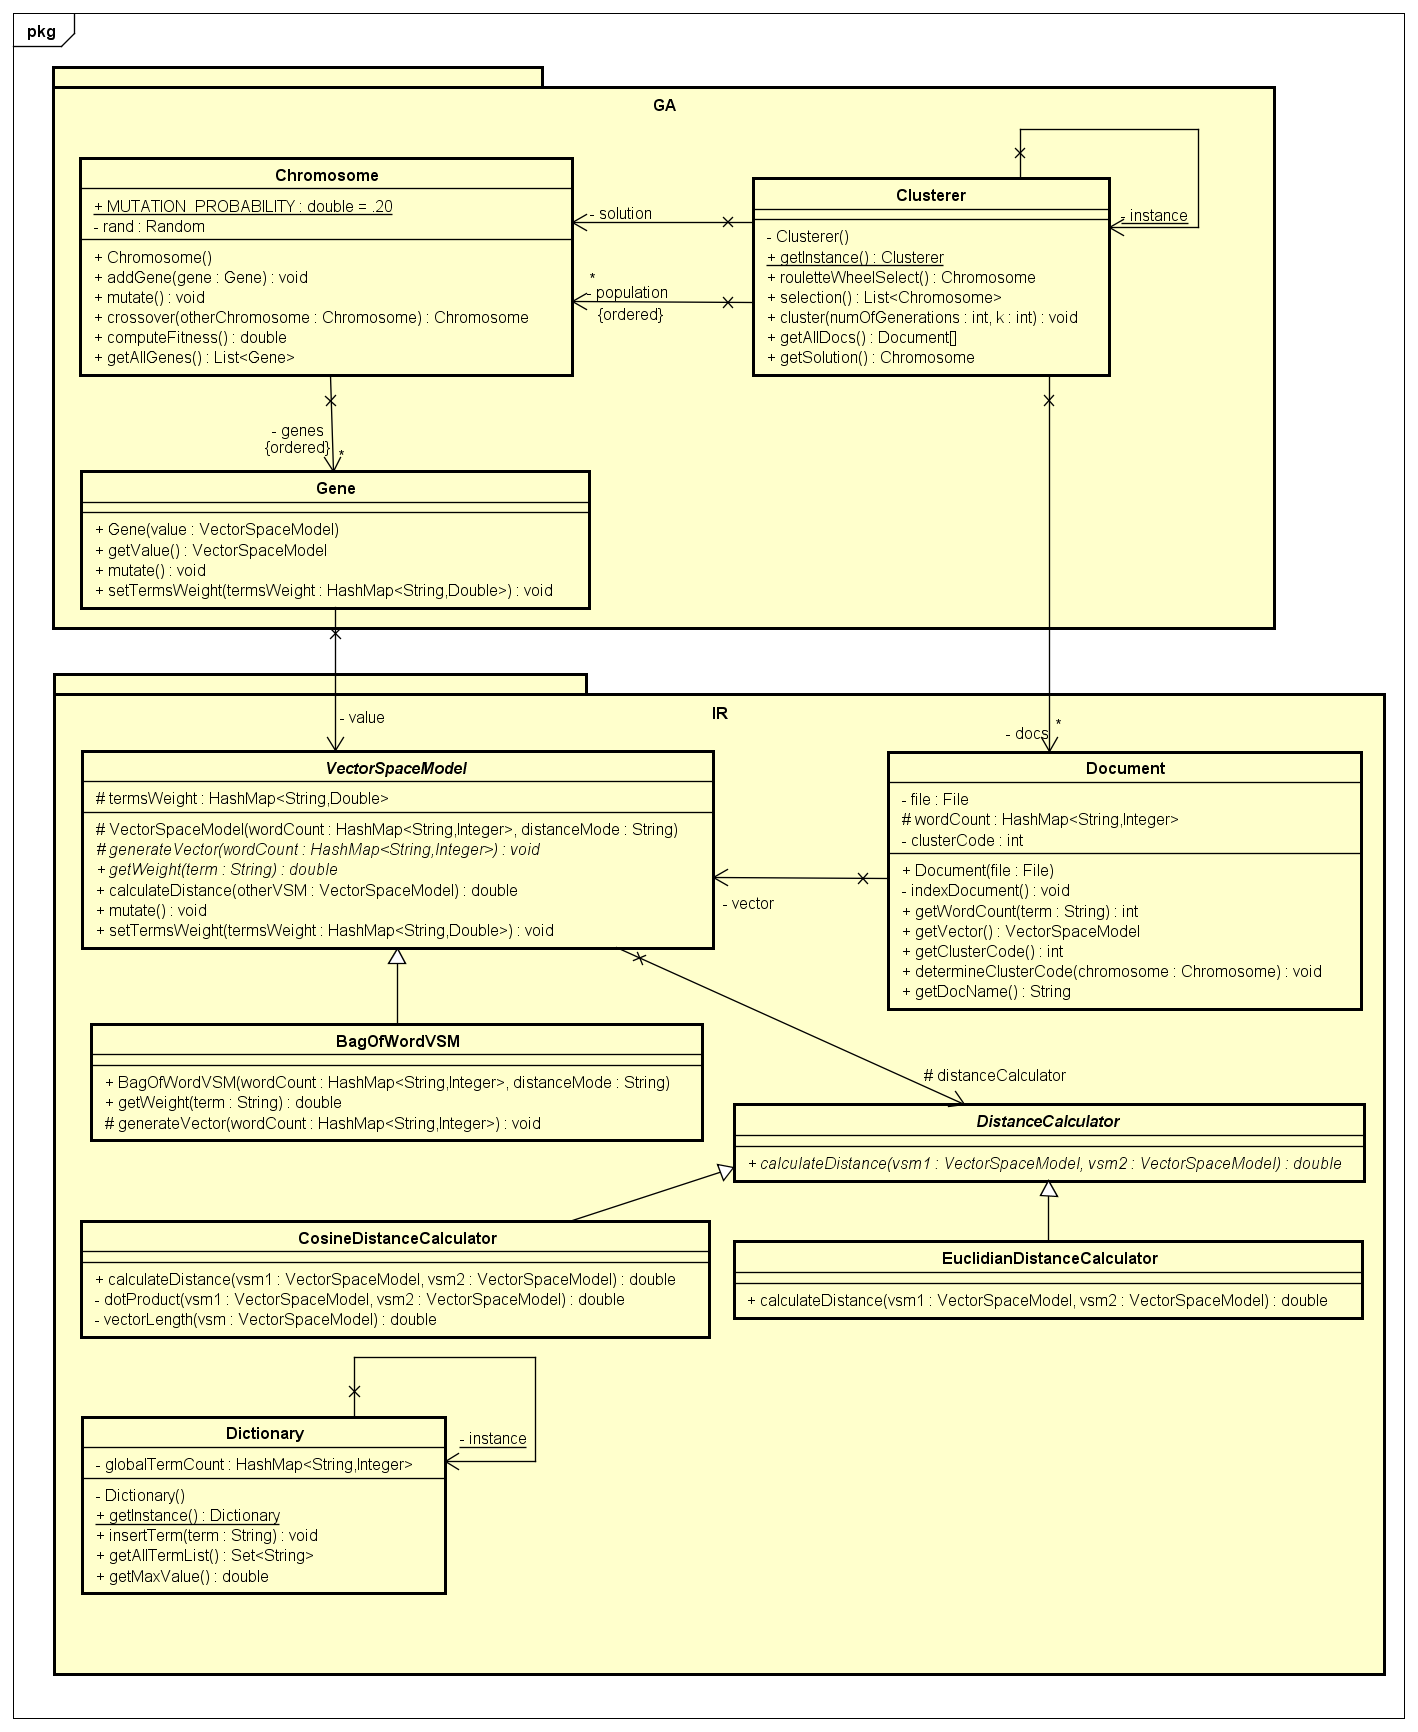
\includegraphics[width=\textwidth]{DiagramKelas}
%		\caption{\textit{Diagram Kelas}}
%		\label{fig:diagramkelas}
%	\end{center}
%\end{figure}

\section{Alur Perangkat Lunak}
Perangkat lunak dibuat untuk dapat mencapai tujuan dari penelitian ini. Sesuai dengan judul penelitian ini, maka perangkat lunak yang dibuat harus bisa mengelompokan dokumen menggunakan algoritma genetika. Oleh karena itu, perangkat lunak dirancang sedemikian rupa sehingga dapat mengolah dokumen masukkan agar dapat menghasilkan keluaran sesuai dengan yang diharapkan. Perangkat lunak yang dibuat memiliki alur seperti yang dijelaskan pada Gambar \ref{fig:software-flow}. 

\begin{figure}[H]
	\centering
	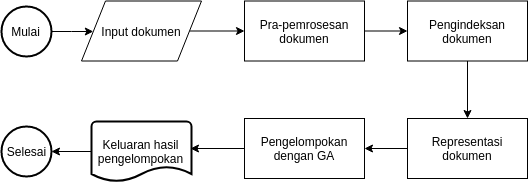
\includegraphics[width=0.7 \linewidth]{Software-flow-diagram}
	\caption{Diagram alur perangkat lunak}
	\label{fig:software-flow}
\end{figure}

Penjelasan dari Gambar \ref{fig:software-flow} adalah sebagai berikut:
\begin{enumerate}
	\item Pertama-tama perangkat lunak akan menerima masukkan berupa koleksi dokumen. Dalam penelitian ini, dokumen-dokumen yang menjadi masukan berasal dari dataset BBC seperti yang telah dijelaskan dalam Subbab \ref{sec:dataset}.
	\item Pra-pemrosesan dokumen diperlukan untuk membersihkan dokumen sehingga tanda baca dan kapitalisasi dapat diabaikan (Subbab \ref{sec:dataset}).
	\item Dokumen kemudian akan diindeks ke dalam suatu \textit{lexicon} yang menampung informasi dari keseluruhan koleksi dokumen. Informasi ini berguna untuk perhitungan bobot TF-IDF (Subbab \ref{sub:analysis:tf-idf}).
	\item Proses selanjutnya adalah merepresentasikan dokumen ke dalam struktur data yang dapat diolah oleh komputer. Dalam penelitian ini dokumen akan direpresentasikan ke dalam bentuk vektor (Subbab \ref{sec:document-rep}).
	\item Pada tahap ini dilakukan operasi-operasi genetik terhadap kromosom mulai dari representasi dokumen (Subbab \ref{sec:chromosome-rep}), inisialisasi populasi (Subbab \ref{sub:analysis:pop-init}), seleksi (Subbab \ref{sub:analysis:selection}), persilangan (Subbab \ref{sub:analysis:crossover}), dan mutasi (Subbab \ref{sub:analysis:mutation}).
	\item Perangkat lunak kemudian akan menghasilkan keluaran sesuai dengan kebutuhan penelitian yang akan dibahas pada Bab \ref{chap:perancangan}.
\end{enumerate}

\section{Evaluasi Hasil Pengelompokan Menggunakan \textit{Purity}}
Seperti yang telah dijelaskan pada Subbab \ref{sec:dataset}, \textit{dataset} yang digunakan merupakan \textit{dataset} berlabel. Untuk mengukur akurasi pengelompokan berdasarkan labelnya, maka pada penelitian ini digunakan pengukuran nilai \textit{purity} (Subbab \ref{sec:purity}). Oleh karena nilai \textit{purity} didapatkan dari membandingkan hasil pengelompokan dengan label \textit{dataset}, maka nilai \textit{purity} ini dapat menjadi acuan kualitas dari hasil suatu pengelompokan. Selain itu, nilai \textit{purity} juga dapat menentukan kinerja dari metrik yang digunakan dalam proses pengelompokan. 
